With higher instantaneous luminosities, triggering on Higgs decays to the
di-lepton final state becomes very challenging. The single lepton triggers can
only be sustained with very tight identification and isolation cuts and fairly 
large momentum thresholds. This leaves only the double lepton triggers as a
viable option for low mass Higgs scenarios. We design the dilepton triggers
to be sufficiently loose that the fake lepton background prediction can be
produced using the dataset collected from the same triggers. The full names
of the triggers used in the analysis are summarized in Table~\ref{tab:triggers}.
We describe the features and motivations for these triggers in Section 
\ref{sec:mainTriggers} below.


\begin{table}[!ht]
  \begin{center}
 {\small
  \begin{tabular} {|l|l|l|c|p{1.0in}|} 
\hline
  Dataset & Trigger name & L1 seed & Run range & Purpose\\
  \hline
  SingleEle & HLT\_Ele27\_CaloIdVT\_CaloIsoT\_TrkIdT\_TrkIsoT\_v1 & L1\_SingleEG15  & 160329-161176 & $ee$, $e\mu$ \\
  SingleEle & HLT\_Ele27\_CaloIdVT\_CaloIsoT\_TrkIdT\_TrkIsoT\_v2 & L1\_SingleEG15  & 161210-161312 & $ee$, $e\mu$ \\
  \hline
  SingleMu & HLT\_IsoMu12\_v1   & L1\_SingleMu7  & 160329-161312 & $\mu\mu$, $e\mu$, efficiency \\
  SingleMu & HLT\_IsoMu17\_v5   & L1\_SingleMu10 & 160329-161312 & $\mu\mu$, $e\mu$, efficiency \\
  SingleMu & HLT\_Mu15\_v2      & L1\_SingleMu10 & 160484-161312 & $\mu\mu$, $e\mu$, efficiency \\
  \hline
  DoubleMu & HLT\_DoubleMu6\_v1 & L1\_DoubleMu3  & 160329-161312 & $\mu\mu$, efficiency\\
  DoubleMu & HLT\_DoubleMu7\_v1 & L1\_DoubleMu3  & 160329-161312 & $\mu\mu$, efficiency \\
  \hline
  DoubleElectron & HLT\_Ele17\_SC8\_M30\_v1\myfootnotemark &  L1\_SingleEG12  & 160329-160877 & efficiency\\ 
  DoubleElectron & HLT\_Ele17\_SC8\_M30\_v2 &  L1\_SingleEG12  & 160888-161312 & efficiency\\ 
  DoubleElectron & HLT\_Ele17\_Ele8\_Loose\_v1\myfootnotemark &  L1\_SingleEG12  & 160329-161176 & $ee$\\ 
  DoubleElectron & HLT\_Ele17\_Ele8\_Loose\_v2 &  L1\_SingleEG12  & 161210-161312 & $ee$\\ 
  DoubleElectron & HLT\_Ele17\_Ele8\_Tight\_v2\myfootnotemark &  L1\_SingleEG12  & 161210-161312 & $ee$\\ 
  DoubleElectron & HLT\_Ele32\_CaloIdL\_CaloIsoVL\_SC17\_v1 & L1\_SingleEG20 & 160329-161176 & $ee$, efficiency\\
  DoubleElectron & HLT\_Ele32\_CaloIdL\_CaloIsoVL\_SC17\_v2 & L1\_SingleEG20 & 161210-161312 & $ee$, efficiency\\
  \hline
  MuEG & HLT\_Mu17\_Ele8\_CaloIdL\_v1 & L1\_Mu3\_EG5 & 160329-161176 & $e\mu$ \\
  MuEG & HLT\_Mu17\_Ele8\_CaloIdL\_v2 & L1\_Mu3\_EG5 & 161210-161312 & $e\mu$ \\
  MuEG & HLT\_Mu8\_Ele17\_CaloIdL\_v1 & L1\_Mu3\_EG5 & 160-161176 & $e\mu$ \\
  MuEG & HLT\_Mu8\_Ele17\_CaloIdL\_v2 & L1\_Mu3\_EG5 & 161210-161312 & $e\mu$ \\
 \hline
  \end{tabular}
}
  \caption{Triggers to be used in the analysis}
   \label{tab:triggers}
  \end{center}
\end{table}
\myfootnotetext{HLT\_Ele17\_CaloIdVT\_CaloIsoVT\_TrkIdT\_TrkIsoVT\_SC8\_Mass30}
\myfootnotetext{HLT\_Ele17\_CaloIdL\_CaloIsoVL\_Ele8\_CaloIdL\_CaloIsoVL}
\myfootnotetext{HLT\_Ele17\_CaloIdT\_TrkIdVL\_CaloIsoVL\_TrkIsoVL\_Ele8\_CaloIdT\_TrkIdVL\_CaloIsoVL\_TrkIsoVL} 
 

\subsubsection{Main analysis triggers}
\label{sec:mainTriggers}

The double electron trigger, {\bf HLT\_Ele17\_CaloIdL\_CaloIsoVL\_Ele8\_CaloIdL\_CaloIsoVL} 
requires two high level trigger electron 
candidates with fairly loose shower shape and calorimeter isolation
requirements on both legs. This is the most challenging channel in terms
of the total rate, due to larger fake electron background rates. To 
accomodate the offline $E_{T}$ selection cuts at $20$ GeV and $10$ GeV
for the leading and trailing leptons, respectively, we require $E_{T}$
cuts of $17$ and $8$ GeV at the HLT level. The leading electron is seeded by the
e/gamma Level-1 non-isolated trigger, L1\_SingleEG12, while the trailing electron
is left unseeded. The cuts imposed on the trigger electrons can be found in 
Table \ref{tab:HLTElectronCuts}, by matching the labels in the trigger name. For 
instantaneous luminosities above 1E33, additional requirements
are needed on the track to cluster matching and track isolation to reduce the 
background rates. The cuts imposed on the electron candidates for the 
tighter version of the dielectron trigger 
{\bf HLT\_Ele17\_CaloIdT\_TrkIdVL\_CaloIsoVL\_TrkIsoVL\_Ele8\_CaloIdT\_TrkIdVL\_CaloIsoVL\_TrkIsoVL }
can be found in Table \ref{tab:HLTElectronCuts}.


\begin{table}[htb]
 \caption{The trigger electron requirements. Values in parentheses corresponds with endcaps when different than in barrel. L=Loose, VL=Very loose.}
 \label{tab:HLTElectronCuts}
 \centering
 \begin{tabular}{|l||c|}
   \hline
   name                       &  criterion \\
   \hline \hline
   \multirow{2}{*}{CaloId\_L} & $\mathrm{H/E < 0.15 (0.10) }$ \\
                               & $\sigma_{\eta\eta}\mathrm{< 0.014\;(0.035)}$ \\
    \hline
    \multirow{2}{*}{TrkId\_VL} & $|\Delta\eta|\mathrm{< 0.01\; (0.01)}$ \\
                               & $\Delta\phi\mathrm{< 0.15\;(0.10)}$  \\
    \hline
    \multirow{2}{*}{CaloIso\_VL} & $\mathrm{ECalIso/E_T <0.2\;(0.2)}$ \\
                                 & $\mathrm{HCalIso/E_T <0.2\;(0.2)}$ \\    
    \hline
    TrkIso\_VL                   & $\mathrm{TrkIso/E_T <0.2\;(0.2)}$ \\

   \hline
 \end{tabular}
\end{table}

 
The double muon trigger, {\bf HLT\_DoubleMu7},  requires two high level trigger 
muon candidates with transverse momentum greater than $7$ GeV. It is seeded 
by the DoubleMu3 Level-1 trigger, with looser quality criteria than the
single muon Level-1 seeds. 
 
In the electron muon channel, we use two complementary triggers, 
{\bf HLT\_Mu17\_Ele8\_CaloIdL} and {\bf HLT\_Mu8\_Ele17\_CaloIdL} requiring
a muon HLT candidate and an electron HLT candidate. The electron
candidate is required to pass the ``Loose'' CaloId requirement as 
summarized in Table \ref{tab:HLTElectronCuts}. These triggers are seeded by 
the Level-1 MuOpen\_EG5 trigger, with minimal requirements on the muon candidate.

Finally, to further recover trigger inefficiencies, we also allow events that 
passed only the single electron 
({\bf HLT\_Ele27\_CaloIdVT\_CaloIsoT\_TrkIdT\_TrkIsoT\_v1} ) or single 
isolated muon ({\bf HLT\_IsoMu17\_v5 } ) triggers. The requirements on the 
electron candidate in the single electron trigger are summarized in 
Table \ref{tab:HLTTightElectronCuts}. 

\begin{table}[htb]
 \caption{The trigger electron requirements for the single electron trigger. 
Values in parentheses corresponds with endcaps when different than in 
barrel. T=Tight, VT=Very tight.}
 \label{tab:HLTTightElectronCuts}
 \centering
 \begin{tabular}{|l||c|}
   \hline
   name                       &  criterion \\
   \hline \hline
   \multirow{2}{*}{CaloId\_VT} & $\mathrm{H/E < 0.05 (0.05) }$ \\
                               & $\sigma_{\eta\eta}\mathrm{< 0.011\;(0.031)}$ \\
    \hline
    \multirow{2}{*}{TrkId\_T} & $|\Delta\eta|\mathrm{< 0.008\; (0.008)}$ \\
                               & $\Delta\phi\mathrm{< 0.07\;(0.05)}$  \\
    \hline
    \multirow{2}{*}{CaloIso\_T} & $\mathrm{ECalIso/E_T <0.15\;(0.075)}$ \\
                                 & $\mathrm{HCalIso/E_T <0.15\;(0.075)}$ \\    
    \hline
    TrkIso\_T                   & $\mathrm{TrkIso/E_T <0.15\;(0.075)}$ \\

   \hline
 \end{tabular}
\end{table}


\subsubsection{Utility triggers}
\label{sec:utilityTriggers}

To measure the electron selection efficiency and the electron trigger
efficiency we use specialized tag and probe triggers designed to maximize
the number of useful \dyll~events for both low and high $p_{T}$ electrons,
while keeping the total trigger rate to a reasonable level. We use 
two different triggers, one specifically for low $p_{T}$ electrons,
{\bf HLT\_Ele17\_CaloIdVT\_CaloIsoVT\_TrkIdT\_TrkIsoVT\_SC8\_Mass30}, 
where very tight identification and isolation cuts are imposed on the 
tag leg to reduce the background rate, and another specifically for
higher $p_{T}$ electrons, {\bf HLT\_Ele32\_CaloIdL\_CaloIsoVL\_SC17}.
The cuts on the tight leg for the low $p_{T}$ trigger is summarized in 
Table \ref{tab:HLTVeryTightElectronCuts}. The cuts on the tight leg
for the high $p_{T}$ triggers can be found in 
Table \ref{tab:HLTElectronCuts}. 

\begin{table}[htb]
 \caption{The trigger electron requirements for the tag leg of the double electron 
tag and probe trigger. Values in parentheses corresponds with endcaps when 
different than in barrel. T=Tight, VT=Very tight.}
 \label{tab:HLTVeryTightElectronCuts}
 \centering
 \begin{tabular}{|l||c|}
   \hline
   name                       &  criterion \\
   \hline \hline
   \multirow{2}{*}{CaloId\_VT} & $\mathrm{H/E < 0.05 (0.05) }$ \\
                               & $\sigma_{\eta\eta}\mathrm{< 0.011\;(0.031)}$ \\
    \hline
    \multirow{2}{*}{TrkId\_T} & $|\Delta\eta|\mathrm{< 0.008\; (0.008)}$ \\
                               & $\Delta\phi\mathrm{< 0.07\;(0.05)}$  \\
    \hline
    \multirow{2}{*}{CaloIso\_VT} & $\mathrm{ECalIso/E_T <0.05\;(0.05)}$ \\
                                 & $\mathrm{HCalIso/E_T <0.05\;(0.05)}$ \\    
    \hline
    TrkIso\_VT                   & $\mathrm{TrkIso/E_T <0.05\;(0.05)}$ \\

   \hline
 \end{tabular}
\end{table}


Another set of specialized triggers are used for recording events
enriched in fake electrons and muons used to measure the lepton fake 
rates. There are two triggers each for electrons and muons with two 
different $p_{T}$ thresholds, in order to collect a sufficiently 
large sample for all $p_{T}$ bins. In order to collect a sample of
events with a fake lepton and a recoiling high $E_{T}$ jet for 
fake rate systematics studies, there are two additional 
triggers for an electron or muon with $p_{T} > 8$~GeV and a jet
with corrected $E_{T}>40$ GeV. Finally to study fake lepton composition
systematics, we use a photon plus electron and a photon plus muon
trigger, where very tight cuts are imposed on the photon to ensure purity. 
The exact cuts imposed on the photon are summarized in 
Table \ref{tab:PhotonPlusLeptonTriggerCuts}.
The full set of triggers and their Level-1 seeds are summarized in 
Table \ref{tab:HWWFakeRateL1Seeds}. These triggers are all prescaled, 
if necessary, to yield a rate of at  least $0.5$Hz each. This rate is 
sufficient to yield a sample of roughly $10^{6}$ events for every 4 
weeks of data taking, enough to make a fake rate measurement with 
small statistical uncertainties. 


\begin{table}[htb]
  \caption{Photon identification criteria. Values in parentheses corresponds 
with endcaps when different than in barrel. VT=Very tight, T=Tight.}
  \label{tab:PhotonPlusLeptonTriggerCuts}
  \centering
  \begin{tabular}{|l||c|}
    \hline
    name                        &  criterion \\
    \hline \hline
    \multirow{2}{*}{CaloId\_VT} & $\mathrm{H/E < 0.05 }$ \\
                                & $\sigma_{\eta\eta}\mathrm{< 0.011\;(0.01)}$ \\
    \hline
    \multirow{3}{*}{Iso\_T}     & $\mathrm{ECalIso} < 5.0 + 0.012*E_{T} $ \\
                                & $\mathrm{HCalIso} < 3.0 + 0.005*E_{T} $ \\
                                & $\mathrm{TrkIso}  < 3.0 + 0.002*E_{T} $ \\
    \hline
  \end{tabular}
\end{table}


\begin{table}[htb]
  \caption{Summary of all lepton fake rate triggers and their Level-1 seeds.}
  \label{tab:HWWFakeRateL1Seeds}
  \centering
  \begin{tabular}{|l||c|}
    \hline
    HLT Path                                  &  L1 Seed       \\
    \hline \hline
    HLT\_Ele8\_CaloIdL\_CaloIsoVL             & L1\_SingleEG5  \\
    HLT\_Ele17\_CaloIdL\_CaloIsoVL            & L1\_SingleEG12 \\
    HLT\_Ele8\_CaloIdL\_CaloIsoVL\_Jet40      & L1\_EG5\_Jet36\_deltaPhi  \\
    HLT\_Photon20\_CaloIdVT\_IsoT\_Ele8\_CaloIdL\_CaloIsoVL & L1\_SingleEG12 \\
    \hline \hline
    HLT\_Mu8                                  &  L1\_SingleMu3  \\
    HLT\_Mu15                                 &  L1\_SingleMu10 \\
    HLT\_Mu8\_Jet40                           &  L1\_Mu3\_Jet20   \\
    HLT\_Mu8\_Photon20\_CaloIdVT\_IsoT        &  L1\_Mu3\_EG5   \\
    \hline
  \end{tabular}
\end{table}



\subsubsection{Trigger efficiency (Tag and probe)}
 
We used the tag and probe method on \dyll~events to provide an unbiased, high-purity, 
lepton sample with which to measure efficiencies.
This method was used successfully by both Tevatron experiments.

Because of the differing kinematics between the \dyll~events and those on which we apply the measured efficiencies,
we split the efficiency measurements into the barrel and endcap regions.
We picked this division because it covers the largest observed variation in efficiency.

We used a single lepton triggered sample available from the Express Stream, 
from which we selected a subset of di-lepton events.
Ultimately we will repeat this using a double lepton triggered sample from the Prompt Reco,
where we select events using one of our tag and probe triggers which are very tight on one lepton,
but loose on the other.

At least one of the leptons, the {\it tag}, was required to pass the full selection criteria criteria 
whilst the other lepton, the {\it probe}, was required to pass a set of identification criteria leaving 
it unbiassed with respect to the criterion under study. 
By requiring that the tag was able to have passed the single lepton trigger on which the events were acquired, 
we reduced the bias due to the trigger on the probe.
Because the analysis uses the same mass window to reduce the \dyll~contribution, 
the tag and probe sample represents an independent control sample.
The tight criteria imposed on the tag coupled with the invariant mass requirement were sufficient to ensure high purity.

To extract the efficiency of offline selection and single trigger efficiency on a per lepton basis, 
we first construct all possible tag-probe pairs in every event.
Because more than one lepton can meet the tag criteria it is possible to use the same event more than once, to find the efficiency

\begin{eqnarray}
\label{eqn:tagAndProbeEfficiencyEqn}
\varepsilon = \frac{2TT + TP}{2TT + TP + TF}.
\end{eqnarray}

Where the event categories are defined as:

\begin{itemize}
	\item 2TT: Both leptons passed the tight criteria, including the trigger. This means that either lepton could be used as a probe, 
	so such events were counted twice.
	\item TP: The probe passed the selection criterion but did not pass the tight criteria.
	\item TF: The probe failed the selection criterion.
\end{itemize}

For the categories to be mutually exclusive it is important to note that the probe definition, 
and the selection criteria studied are always a subset of the tag criteria.
Classifying events and looping over all possible tag-probe combinations are thus equivalent.

To determine the efficiency of the double lepton triggers, we derive the efficiency of the requirements imposed on each leg separately.
This requires a modification to the tag and probe method described above in some cases.
If the trigger objects are saved by the HLT before the requirement that there be two valid objects then
we can check each leg independently of the other using the usual tag and probe method.
If the trigger objects are saved after the requirement that there are two valid objects, then there is 
a 100\% correlation between the decision we can probe on each lepton.
This means that we must pick exactly one tag candidate for each event a priori, which we do 
randomly. 
If the randomly selected tag candidate meets the tight requirements then we are free to 
probe the other lepton.

\subsubsection{Trigger efficiency (Results)}

The tag definition:
\begin{itemize}
	\item  Single trigger blah
	\item Full offline electron/muon selection
\end{itemize}
	
The probe definition (muons / electrons):
\begin{itemize}
	\item  Full offline electron/muon selection
\end{itemize}

  
The per electron efficiency for the seeded leg of the double electron trigger is shown in 
Figure \ref{tab:Ele17Ele8TriggerEfficiencySeededLeg} as a function of $p_{T}$ and $\eta$, 
and summarized in Table \ref{tab:Ele17Ele8TriggerEfficiencySeededLeg}. The efficiency for 
the corresponding unseeded leg is shown in Figure 
\ref{fig:Ele17Ele8TriggerEfficiencyUnseededLeg} and summarized in Table 
\ref{tab:Ele17Ele8TriggerEfficiencyUnseededLeg}. The per electron efficiency for the
single electron trigger is shown in Figure \ref{fig:Ele27Efficiency} and summarized
in Table \ref{tab:Ele27Efficiency}. Finally, to combine these measurements into a final per event
trigger efficiency, one has to fold in the $p_{T}$ and $\eta$ kinematic distributions
of the signal sample.


\begin{table}[!ht]
\begin{center}
\begin{tabular}{|c|c|c|} \hline
              & Barrel ( $|\eta|<1.5$ )  & Endcap ( $|\eta|>1.5$ )  \\ 
\hline
20$<p_{T}<$   & 0.9931 + 0.0012 - 0.0014 & 0.9942 + 0.0019 - 0.0026 \\
\hline
\end{tabular}
\caption{Efficiency for the unseeded leg of the double electron trigger 
separately in bins of $p_{T}$ for the barrel and endcap.
\label{tab:Ele17Ele8TriggerEfficiencySeededLeg}}
\end{center}
\end{table}


\begin{figure}[!h]
\begin{center}
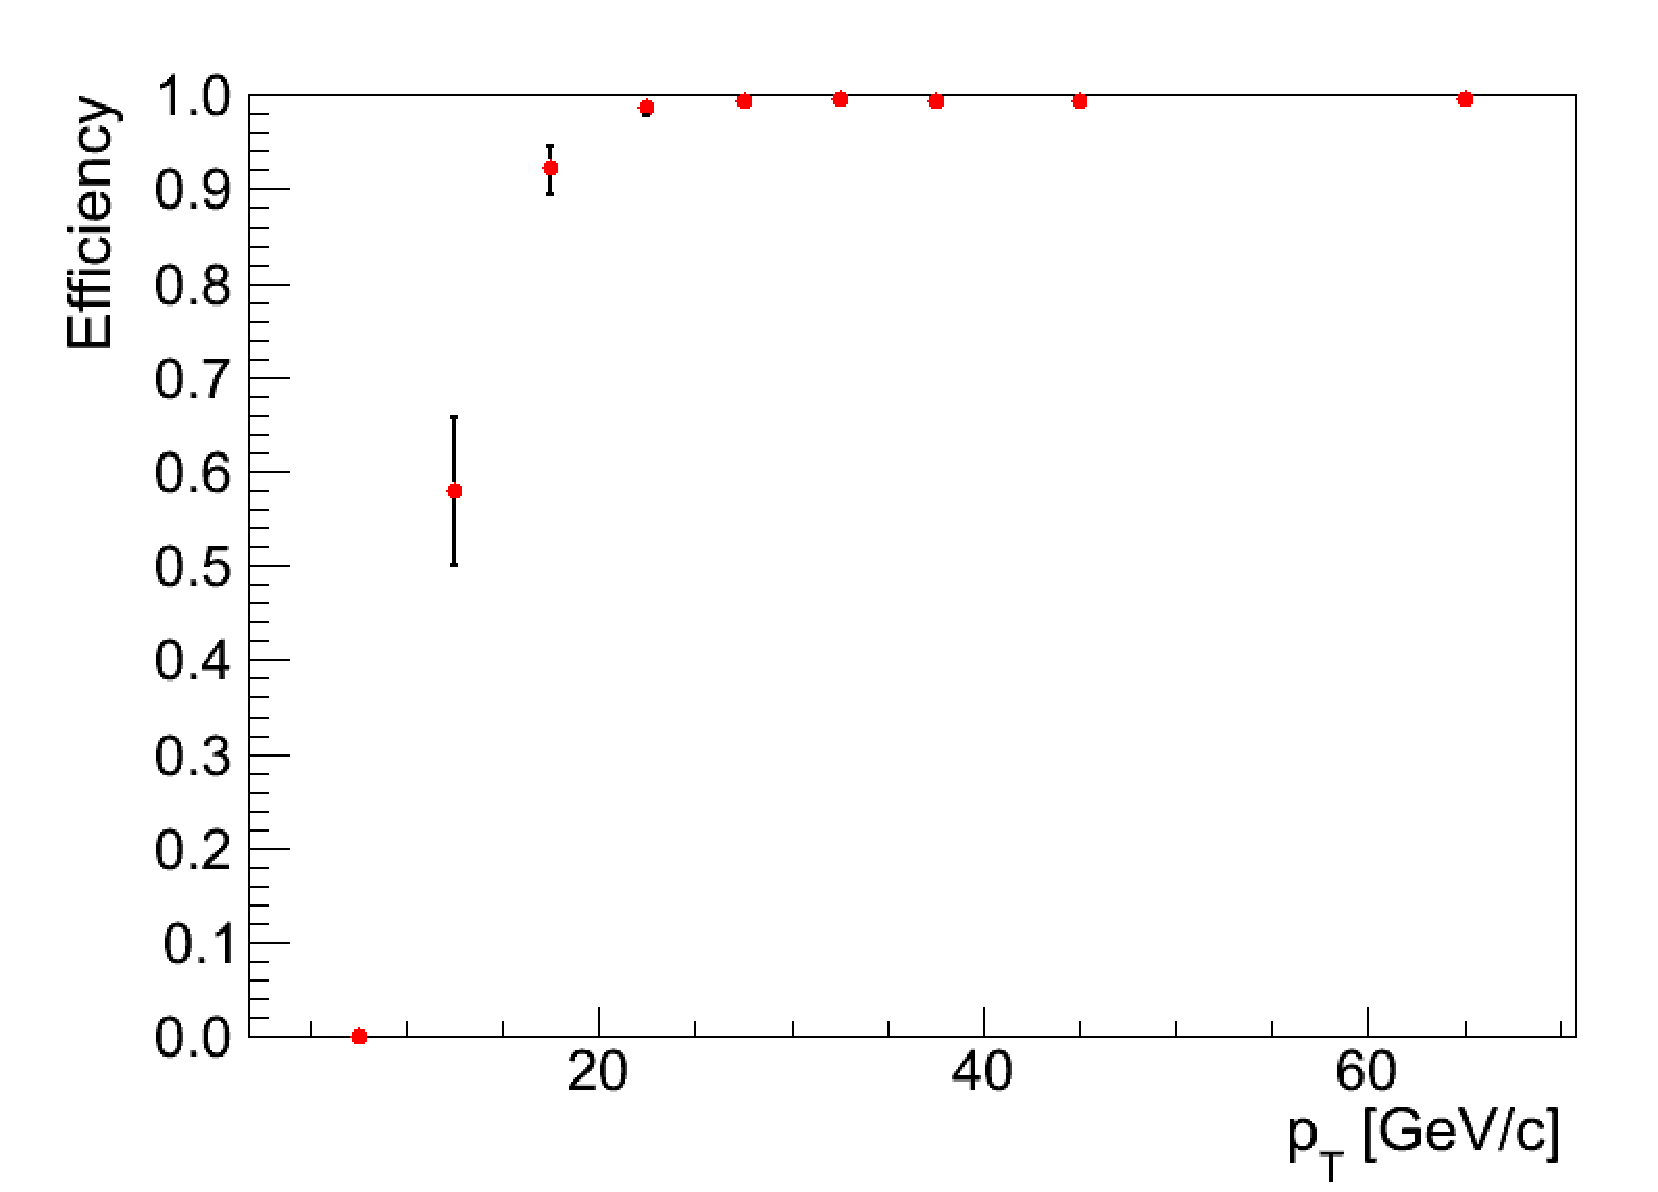
\includegraphics[width=0.48\textwidth]{figures/ElectronTriggerEffVsPt_Ele17Ele8WithL1Seed.pdf}
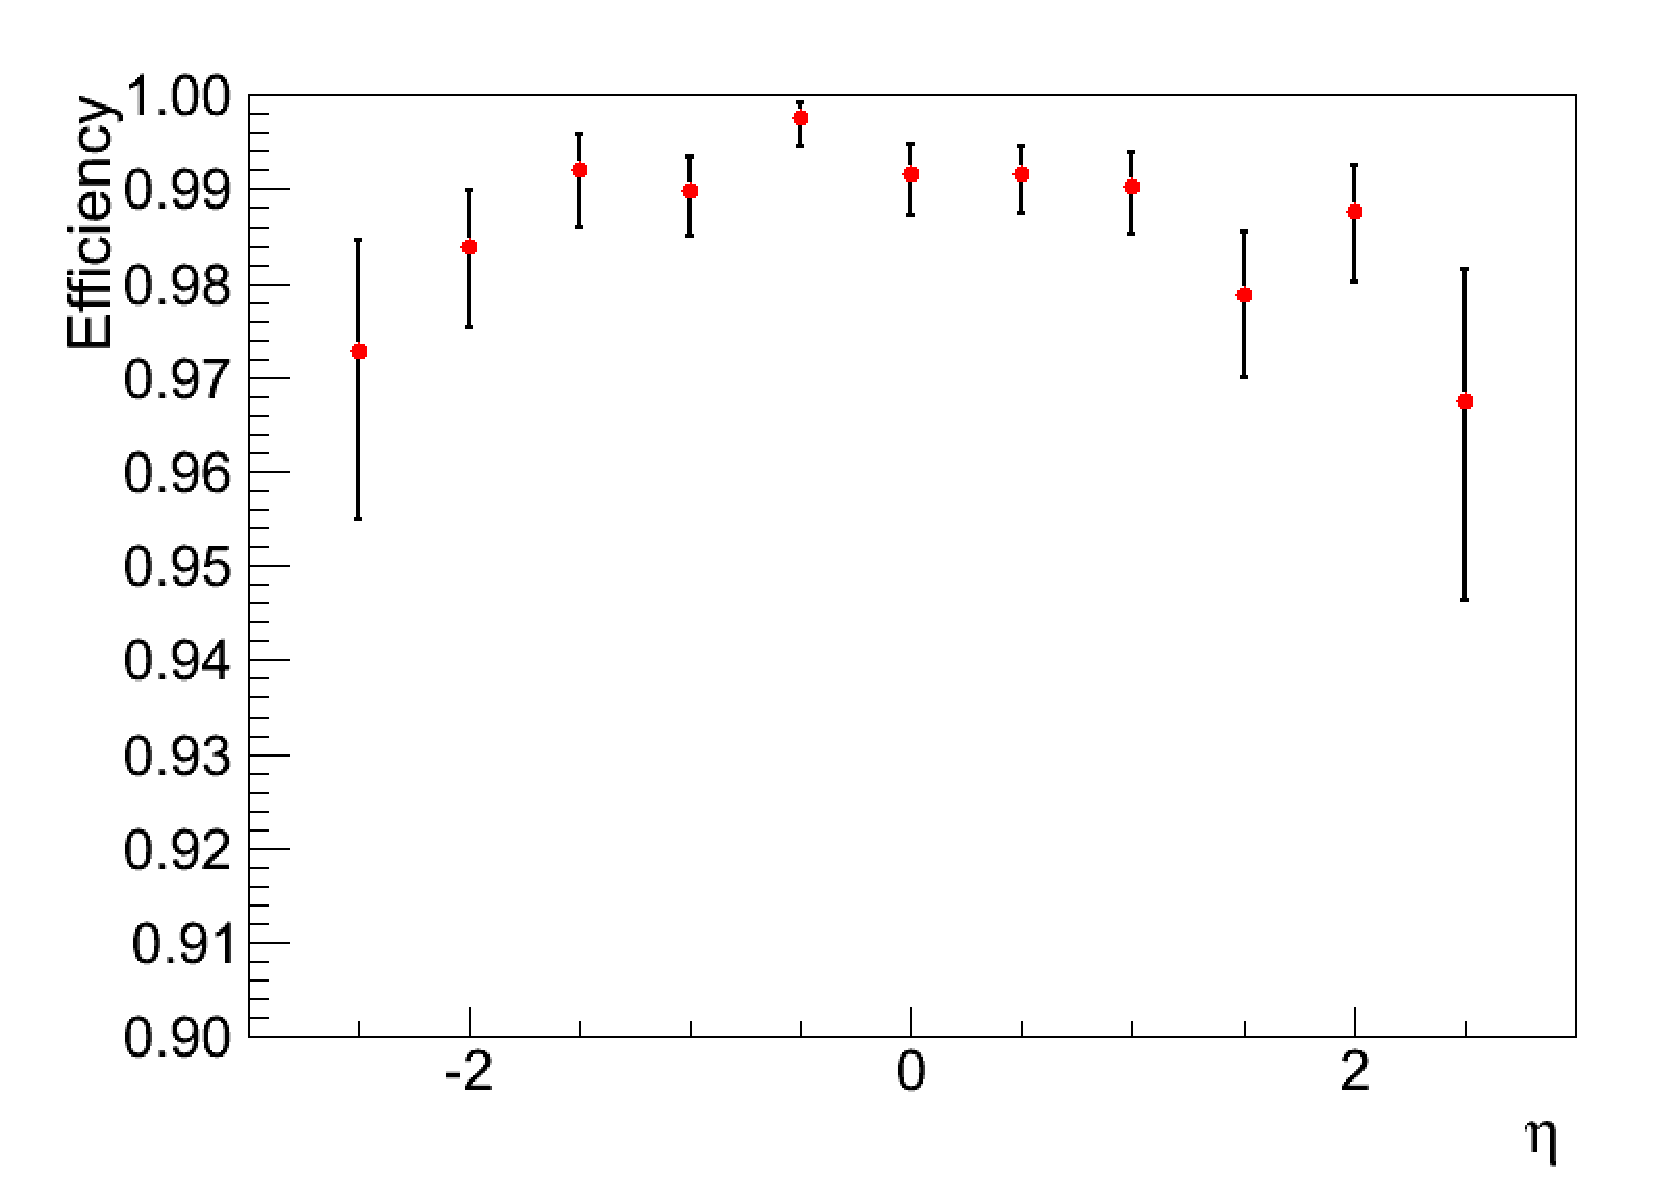
\includegraphics[width=0.48\textwidth]{figures/ElectronTriggerEffVsEta_Ele17Ele8WithL1Seed.pdf}
\end{center}
\caption{Efficiency for the L1 seeded leg of the double electron trigger as a function of $p_{T}$ (a) and $\eta$ (b).}
\label{fig:Ele17Ele8TriggerEfficiencySeededLeg}
\end{figure} 


\begin{table}[!ht]
\begin{center}
\begin{tabular}{|c|c|c|} 
\hline
              & Barrel ( $|\eta|<1.5$ )  & Endcap ( $|\eta|>1.5$ )  \\ 
\hline
10$<p_{T}<$15 & 1.0 + 0.0 - 0.07 & 1.0 + 0.0 - 0.08                 \\
15$<p_{T}<$20 & 1.0 + 0.0 - 0.02 & 0.985 + 0.012 - 0.033            \\
20$<p_{T}<$   & 0.9981 + 0.0006 - 0.0009 & 0.9993 + 0.0005 - 0.0015 \\
\hline
\end{tabular}
\caption{Efficiency for the unseeded leg of the double electron trigger 
separately in bins of $p_{T}$ for the barrel and endcap.
\label{tab:Ele17Ele8TriggerEfficiencyUnseededLeg}}
\end{center}
\end{table}


\begin{figure}[!h]
\begin{center}
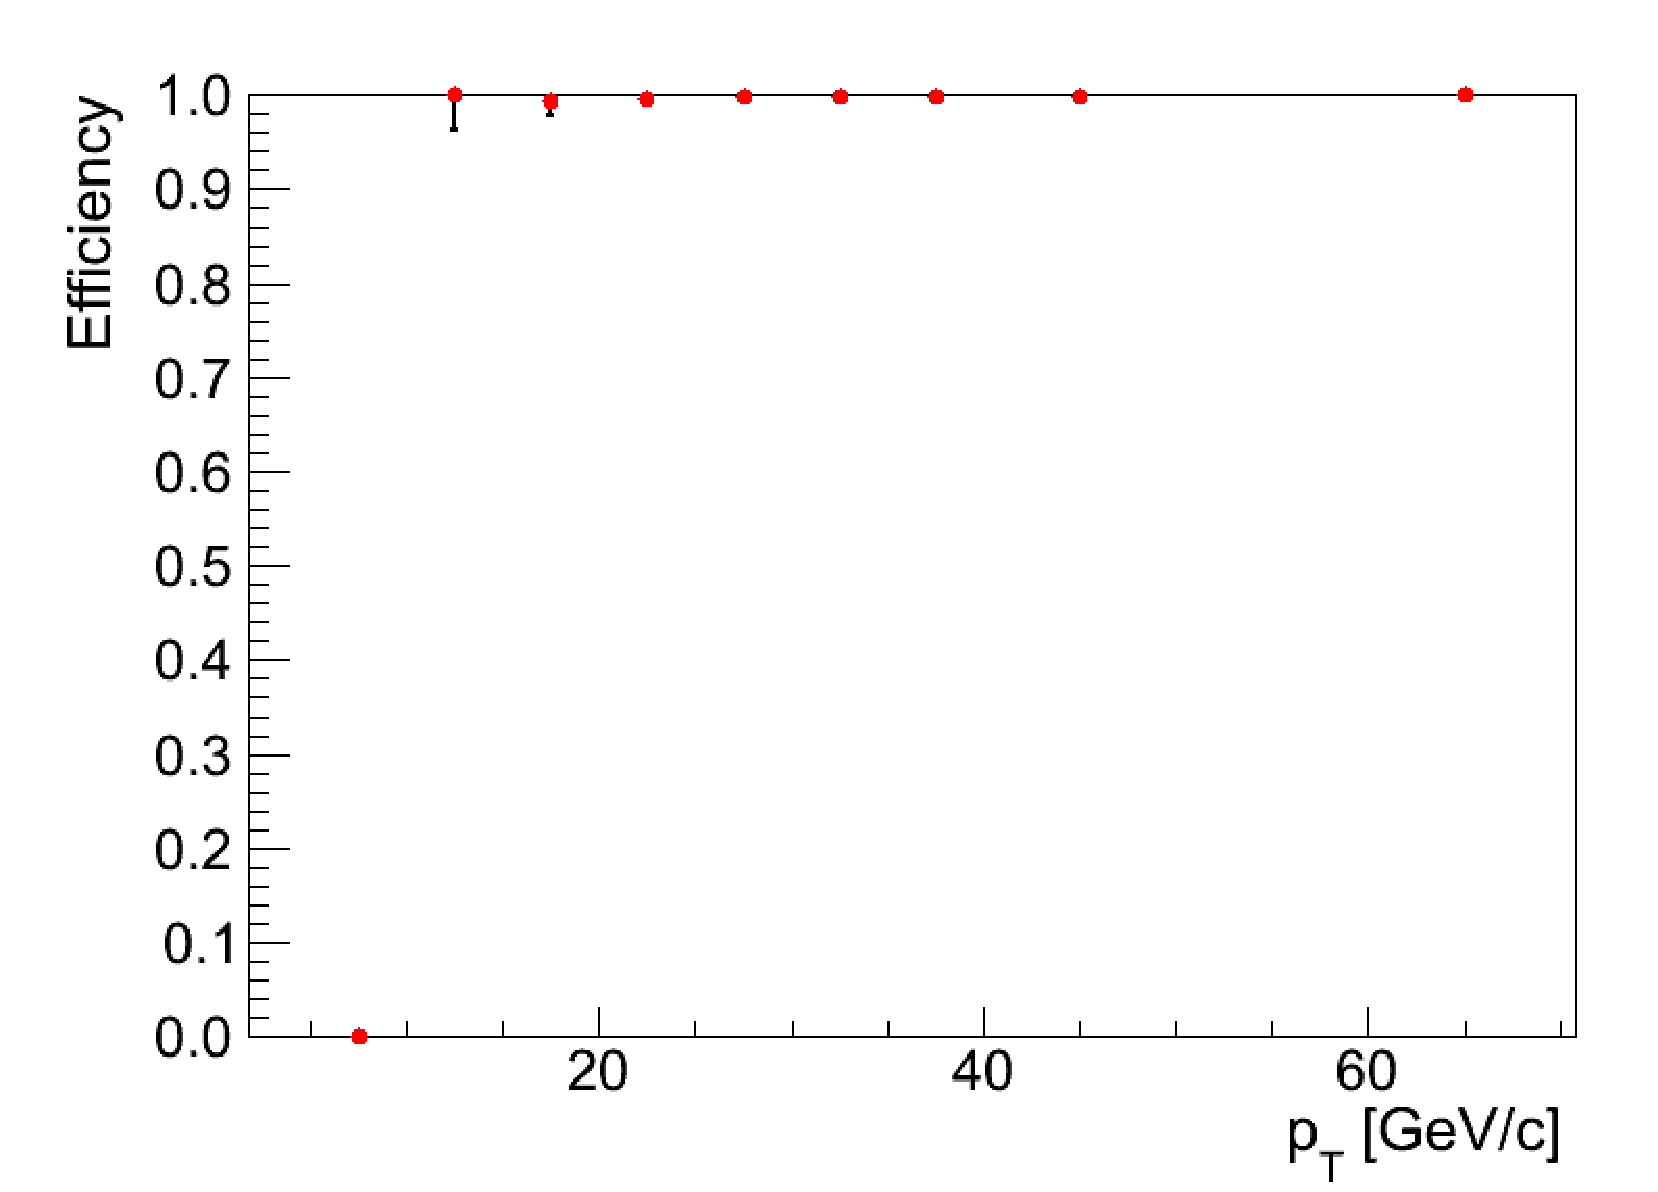
\includegraphics[width=0.48\textwidth]{figures/ElectronTriggerEffVsPt_Ele17Ele8.pdf}
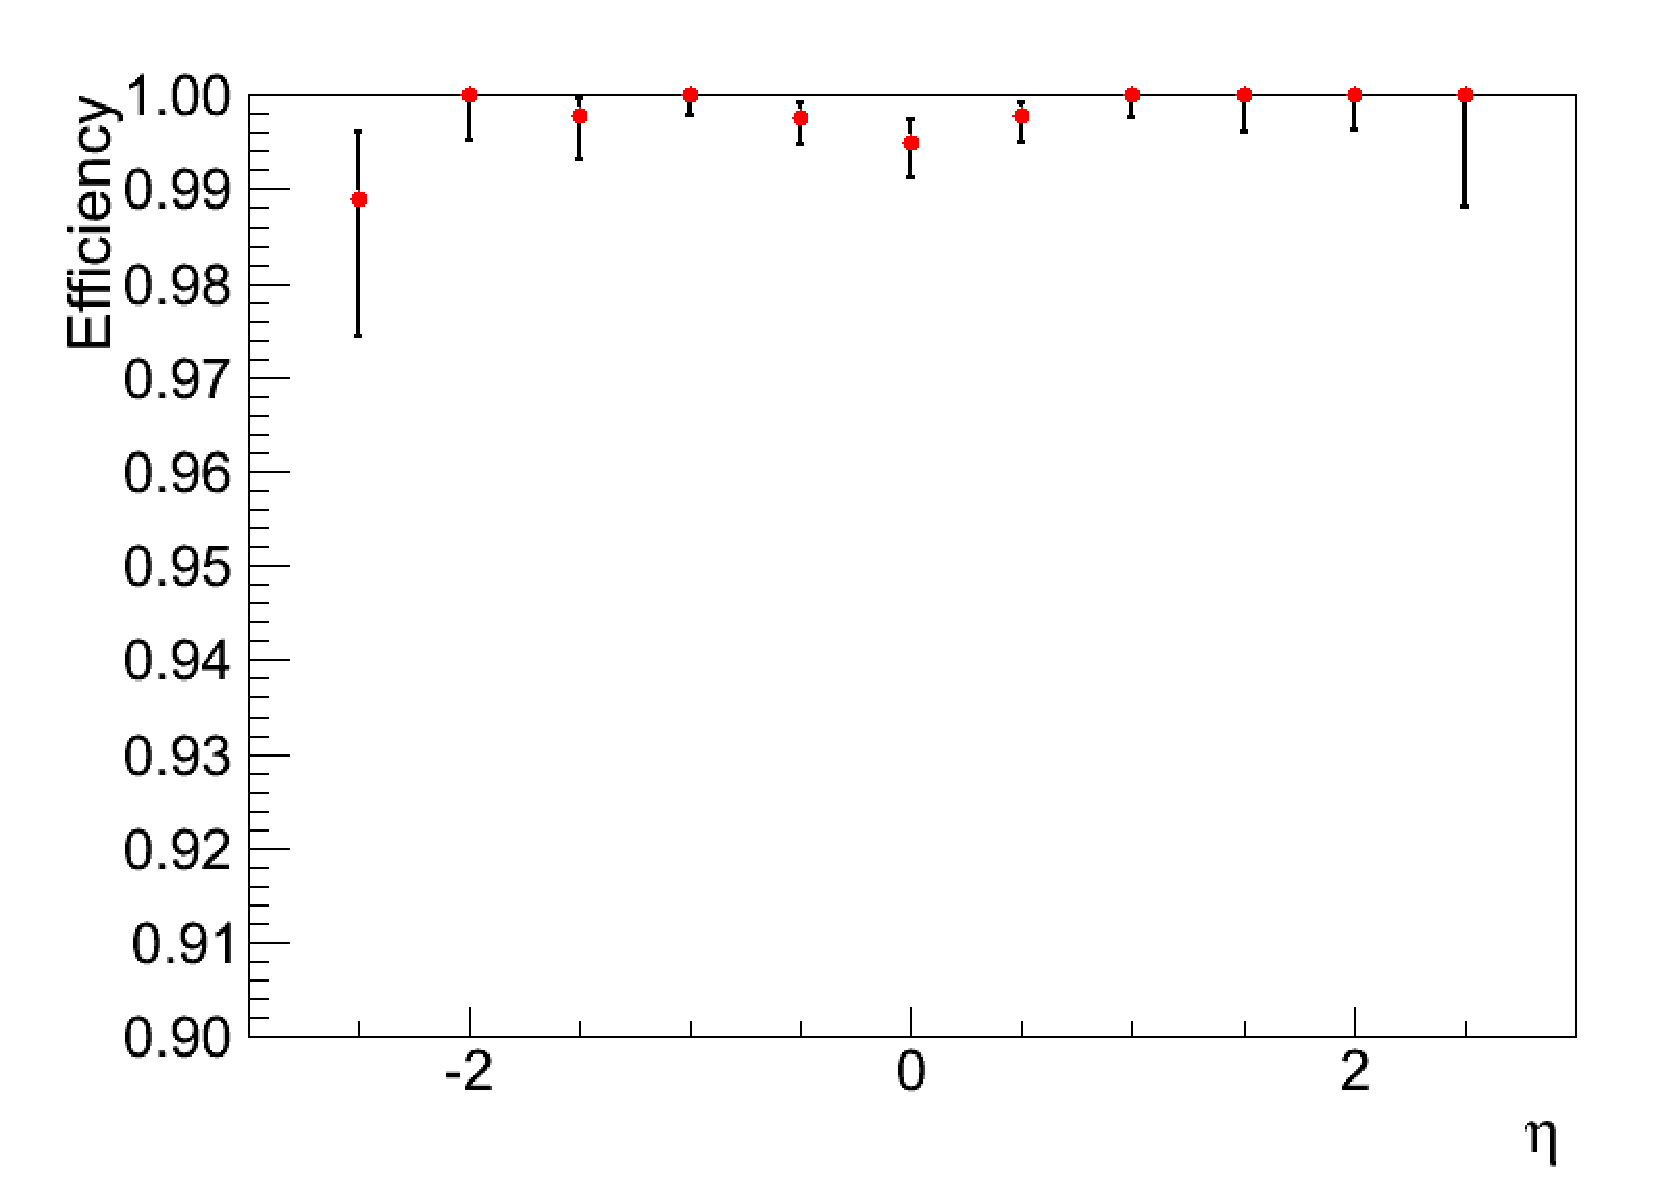
\includegraphics[width=0.48\textwidth]{figures/ElectronTriggerEffVsEta_Ele17Ele8.pdf}
\end{center}
\caption{Efficiency for the unseeded leg of the double electron trigger as a function of $p_{T}$ (a) and $\eta$ (b).}
\label{fig:Ele17Ele8TriggerEfficiencyUnseededLeg}
\end{figure}



\begin{table}[!ht]
\begin{center}
\begin{tabular}{|c|c|c|} \hline
              & Barrel ( $|\eta|<1.5$ )  & Endcap ( $|\eta|>1.5$ )  \\ 
\hline
30$<p_{T}<$   & 0.964 + 0.002 - 0.002 & 0.958 + 0.004 - 0.004 \\
\hline
\end{tabular}
\caption{The single leg efficiency of the single electron trigger 
separately in bins of $p_{T}$ for the barrel and endcap.
\label{tab:Ele27Efficiency}}
\end{center}
\end{table}


\begin{figure}[!h]
\begin{center}
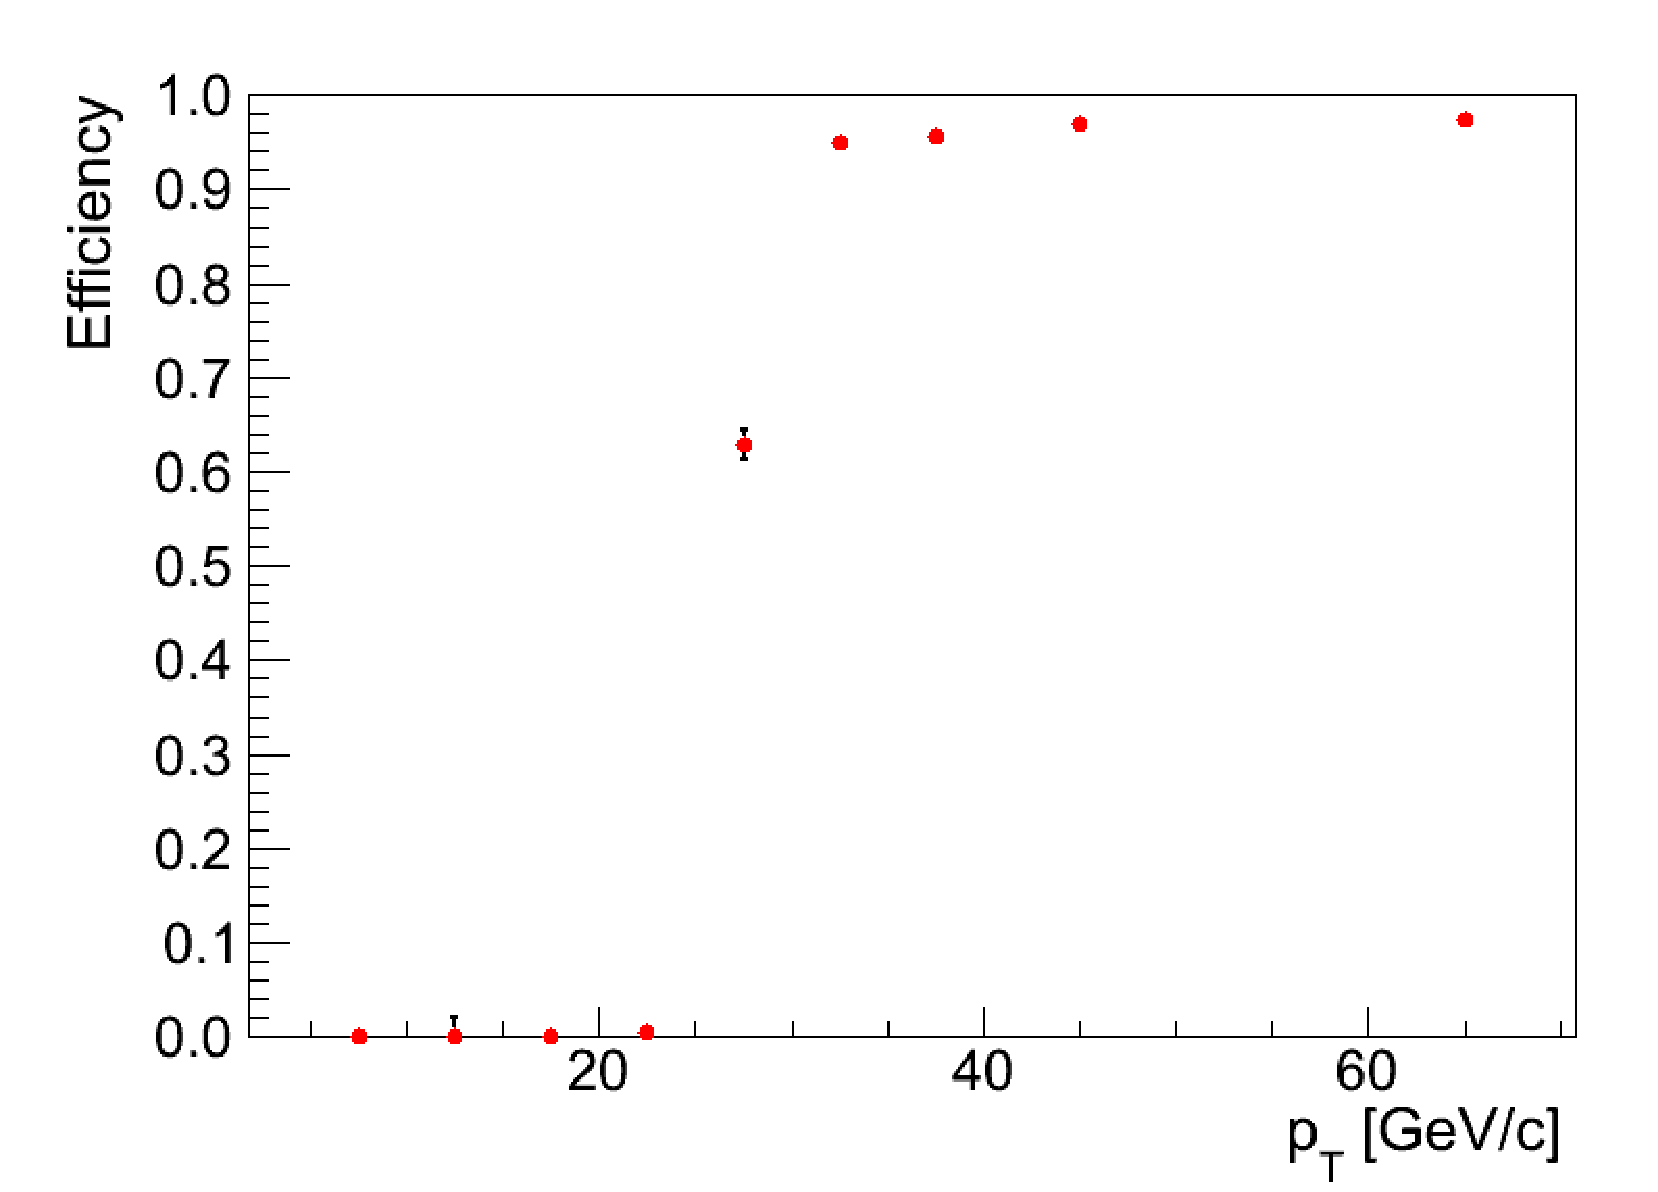
\includegraphics[width=0.48\textwidth]{figures/ElectronTriggerEffVsPt_Ele27Tight.pdf}
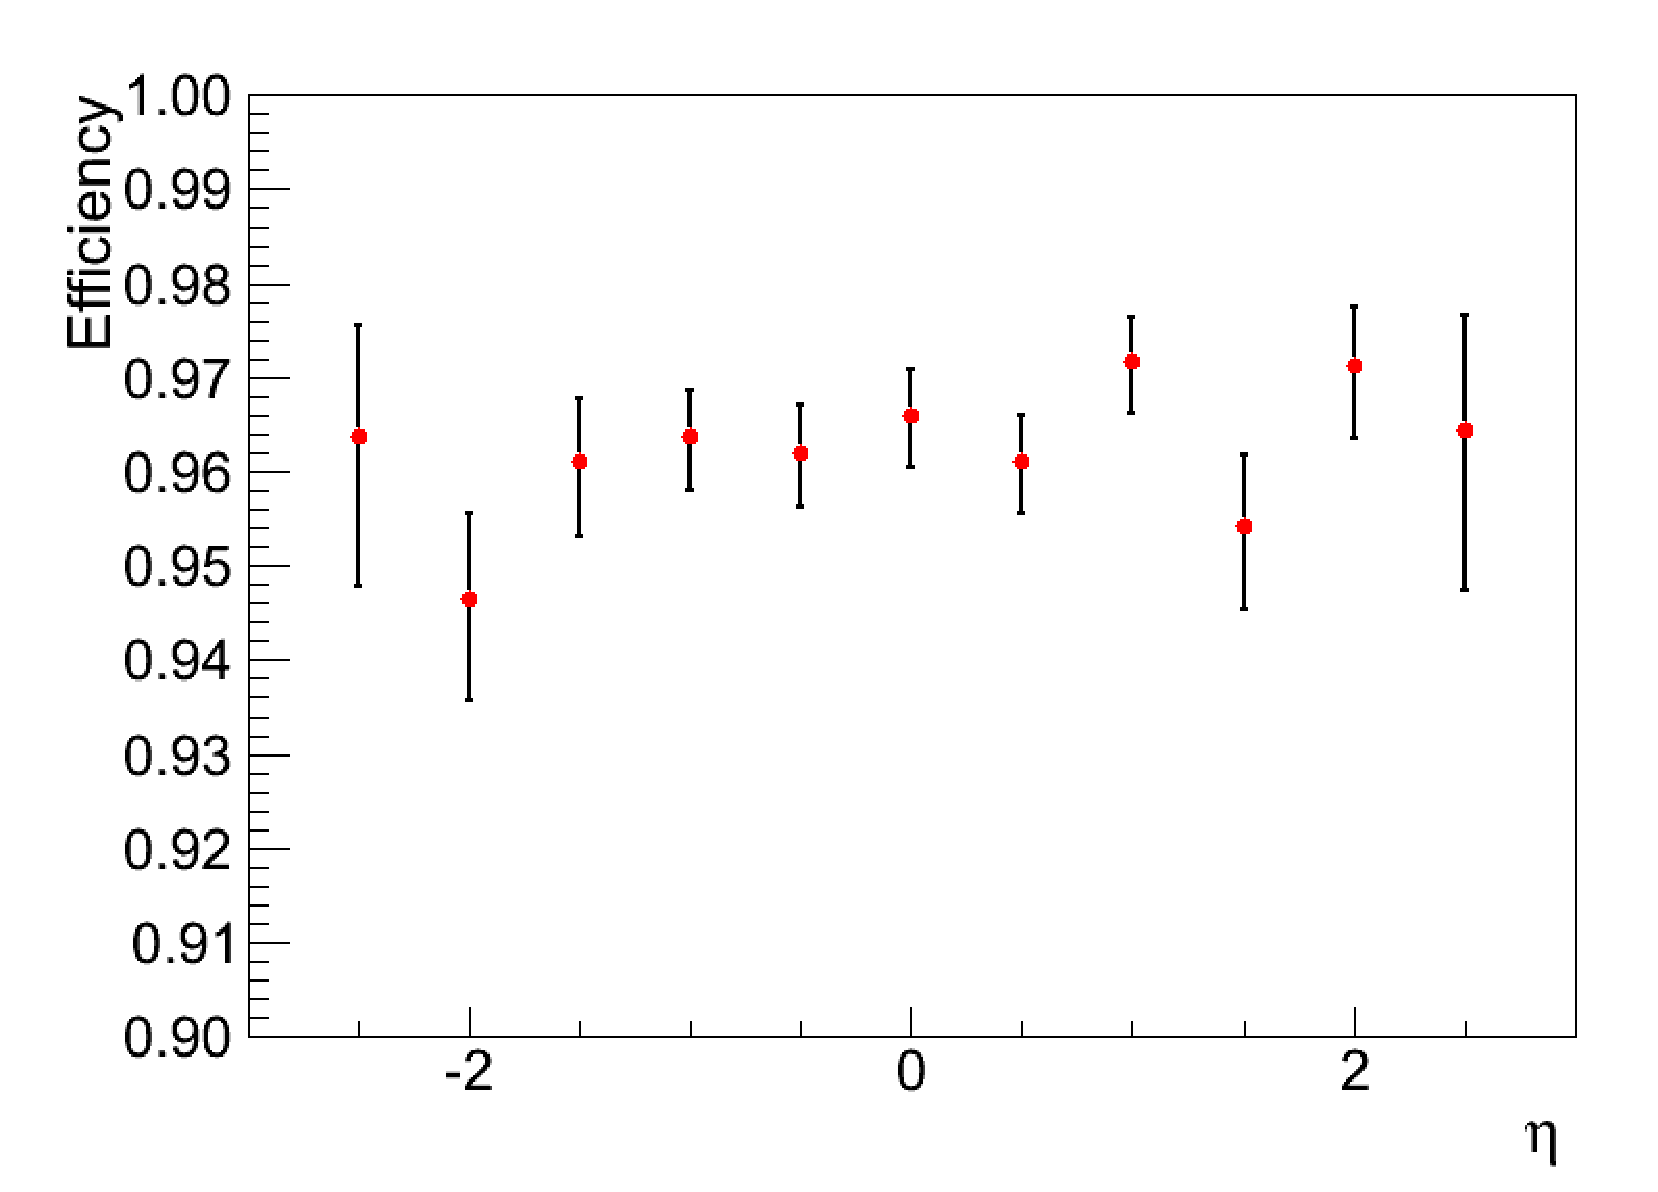
\includegraphics[width=0.48\textwidth]{figures/ElectronTriggerEffVsEta_Ele27Tight.pdf}
\end{center}
\caption{The single leg efficiency of the single electron trigger as a function of $p_{T}$ (a) and $\eta$ (b).}
\label{fig:Ele27Efficiency}
\end{figure}





%% DoubleMu7 Express : 
%% Pt10To15:
%% Barrel Eff : 25/26 = 0.961538 + 0.0318235 - 0.0828584
%% Endcap Eff : 19/20 = 0.95 + 0.0413792 - 0.105642

%% Pt15To20:
%% Barrel Eff : 81/83 = 0.975904 + 0.015537 - 0.0308607
%% Endcap Eff : 51/54 = 0.944444 + 0.0300568 - 0.051037

%% Pt20ToInf:
%% Barrel Eff : 5012/5247 = 0.955213 + 0.00285777 - 0.00303673
%% Endcap Eff : 1906/2044 = 0.932485 + 0.0055673 - 0.00600819

%% DoubleMu7 Prompt Reco : 
%% Pt10To15:
%% Barrel Eff : 33/35 = 0.942857 + 0.0367943 - 0.0703594
%% Endcap Eff : 40/43 = 0.930233 + 0.0376956 - 0.0631583

%% Pt15To20:
%% Barrel Eff : 107/108 = 0.990741 + 0.00765718 - 0.0209429
%% Endcap Eff : 82/83 = 0.987952 + 0.00996406 - 0.0271254

%% Pt20ToInf:
%% Barrel Eff : 5471/5666 = 0.965584 + 0.00242228 - 0.00259228
%% Endcap Eff : 2085/2181 = 0.955983 + 0.00439809 - 0.00483715


%% SingleMu24 Express:
%% Pt20ToInf:
%% Barrel Eff : 6345/6815 = 0.931034 + 0.00307405 - 0.00320332
%% Endcap Eff : 1412/1637 = 0.862553 + 0.00857366 - 0.00903148

%% SingleMu24 PromptReco
%% Pt20ToInf:
%% Barrel Eff : 6713/7233 = 0.928107 + 0.00304181 - 0.00316265
%% Endcap Eff : 1436/1665 = 0.862462 + 0.0085031 - 0.00895298


\subsubsection{Offline efficiency (Results)}

The tag definition:
\begin{itemize}
	\item  Single trigger blah
	\item Full offline electron/muon selection
\end{itemize}
	
The probe definition (muons / electrons):
\begin{itemize}
	\item  Full offline electron/muon selection
\end{itemize}

Repeat as above for each measurement, and discussions of systematics etc.


